%                                                                 aa.dem
% AA vers. 9.1, LaTeX class for Astronomy & Astrophysics
% demonstration file
%                                                       (c) EDP Sciences
%-----------------------------------------------------------------------
%
%\documentclass[referee]{aa} % for a referee version
%\documentclass[onecolumn]{aa} % for a paper on 1 column  
%\documentclass[longauth]{aa} % for the long lists of affiliations
%\documentclass[letter]{aa} % for the letters
%\documentclass[bibyear]{aa} % if the references are not structured
%                              according to the author-year natbib style

%
\documentclass[letter]{aa}  

%
\usepackage{graphicx}
%%%%%%%%%%%%%%%%%%%%%%%%%%%%%%%%%%%%%%%%
\usepackage{txfonts}
%%%%%%%%%%%%%%%%%%%%%%%%%%%%%%%%%%%%%%%%
\newcommand{\mycomment}[1]{}

%
\begin{document}


\title{A Presentation of Galaxies with Polar Structures}

\titlerunning{The occurrence rate of polar structures}

\author{A.V. Mosenkov\inst{1} \and C.M. Garrett\inst{1}
          }


\institute{Department of Physics and Astronomy, N283 ESC, Brigham Young University, Provo, UT 84602, USA}
\date{Received November, 2023; accepted ???, 2023}

\abstract{Certain galaxies exist that exhibit kinematically and photometrically decoupled systems that are inclined to an extreme angle as compared to the major planar axis of the host galaxy. Historically, these have been identified and studied, however, they are quite rare and difficult to catalogue. In this work, I examined a sample of over 10,000 galaxies from the Sloan Digital Sky Survey (SDSS) Strie \,82 for the presence of galaxies with these polar structures described. With the deep SDSS Stripe \,82, the DESI Legacy Imaging Surveys, and the Hyper Suprime-Cam Subaru Strategic Program, 143 exceptional candidates with polar structures were found. The results indicate that the occurrence rate for which polar structures are found in galaxies is underestimated, and may total to 1.43\%}

\keywords{galaxies: structure -- galaxies: elliptical and lenticular -- galaxies: formation -- galaxies: evolution}

\maketitle
\nolinenumbers

%
%________________________________________________________________

\section{Introduction} 
\label{sec:intro}

Polar-ring galaxies (PRGs) were identified first in a series of studies by \citet{1978AJ.....83.1360S}, \citet{1978ApJ...226L.115B}, and \citet{1983AJ.....88..909S}, and are a rare type of galaxy that has a pronounced ring of stars and gas orbiting nearly orthogonal to the plane of the host galaxy. A more generalized class of polarized galactic structures were proposed which made space for polar/tilted discs, \citep{1999ApJ...519L.127B,2020MNRAS.497.2039M}, polar bulges \citep{2012MNRAS.423L..79C,2015AstL...41..748R}, halos that are perpendicular to the disc \citep{2016ApJ...823...19C,2020MNRAS.494.1751M,2021MNRAS.506.5030M}, and tidally disrupted material from nearby satellites \citep{2010AJ....140..962M,2019A&A...632L..13M,2023A&A...671A.141M}. The class of polar structures has proven useful in exploring properties of dark matter \citep{1987ApJ...314..439W,1994ApJ...436..629S,1996A&A...305..763C,2003ApJ...585..730I,2011MNRAS.418..244M,2012MNRAS.425.1967S,2014MNRAS.441.2650K,2015BaltA..24...76M} as well as galactic accretion dynamics \citep{2008ApJ...689..678B} and merger events \citep{1998ApJ...499..635B,2003A&A...401..817B}. To date, PRGs are generally understood to form from tidal accretion events, where matter from a donor galaxy is given to the host \citep[][]{schweizer1983colliding,1997A&A...325..933R} which also includes the disruption of a (gas-rich) satellite into the plane perpendicular of the host \citep{1991wdir.conf..112R,1992ApJ...389L..55K}, major mergers of galaxies \citep[][]{bekki1997formation,bekki1998formation,2003A&A...401..817B}, and lastly, cosmological filament accretion \citep{2006ApJ...636L..25M,2008ApJ...689..678B}. Modern simulations conform the possibility of these structures forming in any of these manners (\citealt{2019MNRAS.485..464L,2021MNRAS.504.5702W,2023arXiv231018597S}). While past catalogues of PRGs have experienced severe limitations in their photometric depth, more modern observations have allowed  for much more careful analysis of structures previously unidentifiable. While it is unfortunate that many of these galaxies have very low average surface brightness, which has caused variance in predicted occurrence rates (See \citet{reshetnikov2011polar}, \citet{2019MNRAS.483.1470R}), polar structures are still discernible with deep imaging from the Sloan Digital Sky Survey. In this article, we aim to continue the study by \citet{mosenkov2022unveiling}, adding to (\citet{2024AstL...}) and the examination of Stripe\,82 data to identify additional, previously unrecognised galaxies with polar rings. Surprisingly, we have found a total of 143 galaxies with polar rings, polar bulges and polar halos, many more than previously spotted using regular imaging, demonstrating that PRGs are more common than expected. 

\section{Data and sample selection}
\label{sec:data}
%my version
A sample of 10,000 galaxies was obtained from the Siena Galaxy Atlas (\cite{siena}), which is a compilation of of galaxies using the Hyperleda database. The galactic sample was randomly selected from the database. All of the images from the Siena Galaxy Atlas were downloaded from the DESI Legacy Survey and enhanced using the method described in \citet{2024AstL...}. We note that the results of this classification are preliminary because they may be subject to our erroneous interpretation of the observed structures, so a quantitative analysis of the selected objects by means of host+ring decomposition (similar to that in \citealt{mosenkov2022unveiling}) will be performed in a subsequent work. In this paper, this classification is provided only for reference, and we do not use this separation into sub-classes in the following sections. 
Here, we focus only on the statistics of polar rings or related objects, whereas in future paper, we will present an atlas of all selected candidates for galaxies with polar structures and explore their morphological features in detail. In Fig.~\ref{fig:examples}, we present typical examples of candidates for galaxies with polar structures from the selected sample\footnote{Mosaic images for all candidates, along with their coordinates, are available in the supplementary material.}.


\begin{figure*}
    \centering
    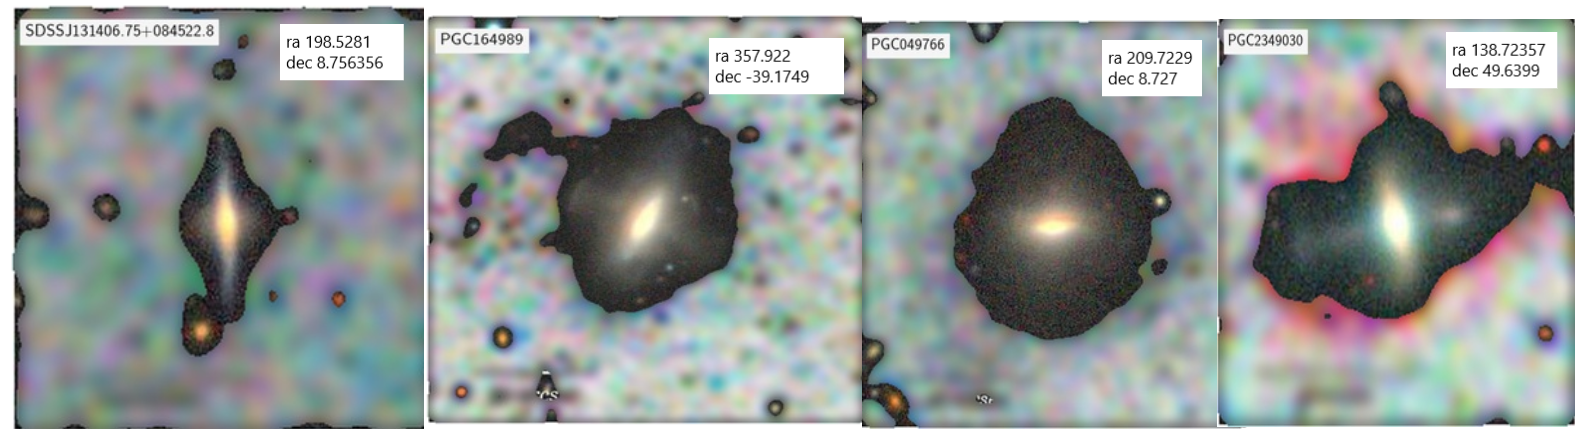
\includegraphics[width = .87\paperwidth]{Images/myimages.png}
    \caption{Examples of candidates for galaxies with polar structures from our sample as seen in the DESI Legacy from left to right: a polar bulge structure, another galaxy with a polar bulge, a polar-halo galaxy, and a galaxy forming another polar bulge structure. The coordinates for each galaxy are given in the upper right corner of each plot, with the reference name in the upper left. }
    \label{fig:examples}
\end{figure*}



\section{Results and discussion}
\label{sec:properties}

\begin{figure*}
\centering
    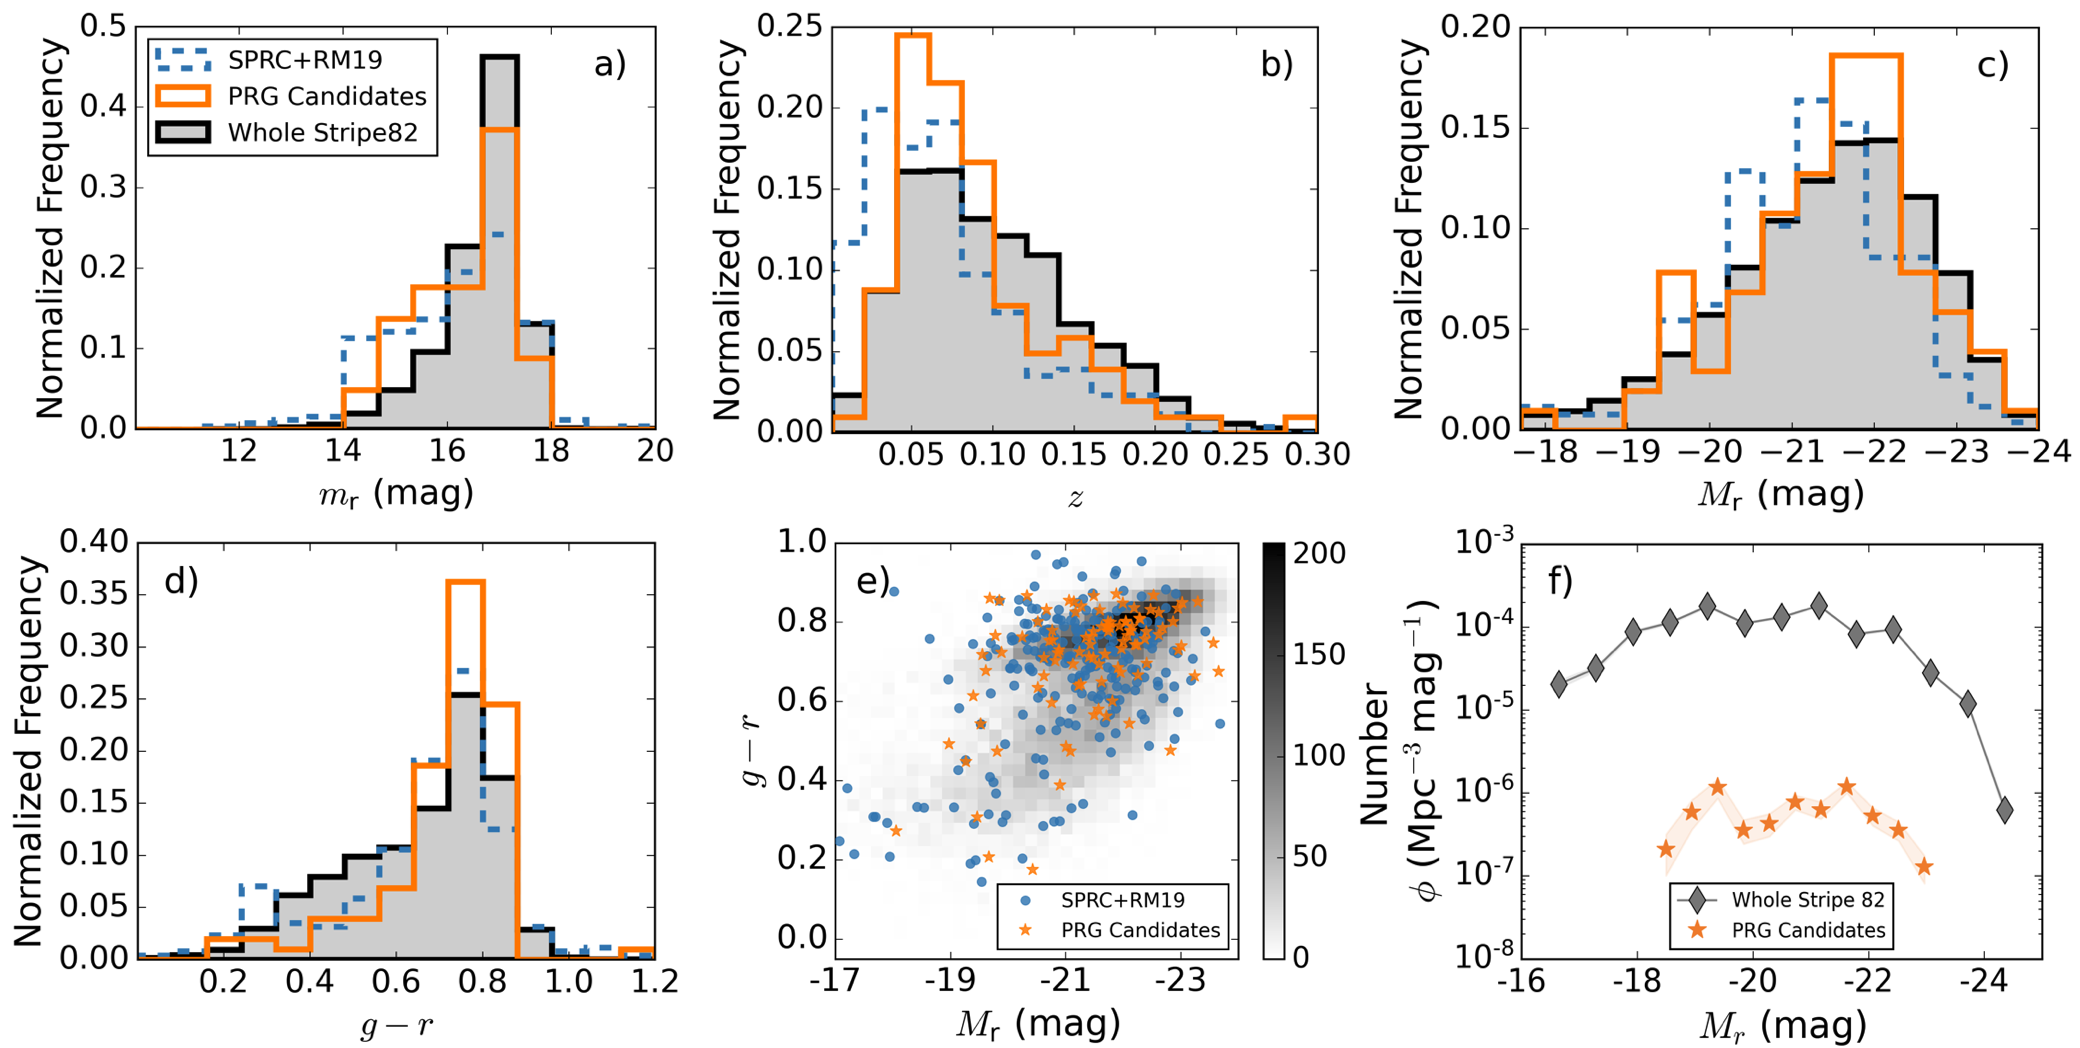
\includegraphics[width = \linewidth]{Images/all_plots.png}
    \caption{Normalized histograms comparing {\it a)} apparent magnitude in the $r$ band, {\it b)} redshift $z$, {\it c)} absolute magnitude in the $r$ band, and {\it d)} galaxy colour $g-r$. The black filled histograms represent the entire Stripe\,82 sample, while the SPRC+RM19 (see text)
    and our new candidates are shown as blue dashed and orange solid histograms, respectively. Plot {\it e)}: a colour-magnitude diagram (the underlying density plot depicts the distribution of the entire Stripe\,82 sample of the 18,362 galaxies). All magnitudes have been corrected for K-correction \citep{2010MNRAS.405.1409C,2012MNRAS.419.1727C} and Galactic extinction using the conversions from \citet{2011ApJ...737..103S} applied to $E(B-V)$ from \citet{1998ApJ...500..525S}. Plot {\it f)}: luminosity functions of our new PRG sample and the entire Stripe\,82 sample calculated with Cho\l{}oniewski's method \citep{1986MNRAS.223....1C}.}
    \label{fig:all_plots}
\end{figure*}

Out of 10,000 galaxies, 143 total were labeled as exhibiting polar structures. This is consistent with \citet{2024AstL...}, where they gave an approximate value of 1-3\%. The best polar structures are presented in Figure \ref{fig:examples}. Polar structures can be formed in a variety of different methods. 
Firstly, polar structures can form via tidal accretion. As two galaxies interact gravitational, polarities can form \ref{fig:tidalacc}.
\begin{figure}
\centering
    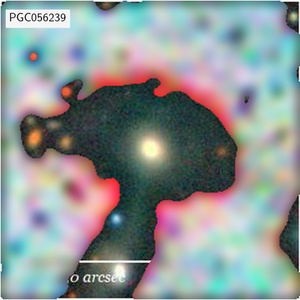
\includegraphics[scale = 0.7]{Images/PGC056239.jpg}
    \caption{A demonstration of tidal accretion-- the target galaxy PGC 56239 is see to gain material from a neighbor, which forms a structure perpendicular to the plane of the galaxy. }
    \label{fig:tidalacc}
\end{figure}
Secondly, polar structures have been observed to form as repercussions of major merging. Extreme gravitational interactions yield such structures as can be viewed in \ref{fig:major}.
\begin{figure}
    \centering
    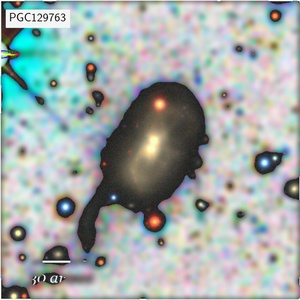
\includegraphics[scale = 0.7]{Images/PGC129763.jpg}
    \caption{A major merger is depicted, and polar structures are visible in all directions from the combining cores.}
    \label{fig:major}
\end{figure}
Thirdly, we can observe polar structures observe in starburst events. As gravitational perturbations or other phenomena trigger star burst in the host galaxy, either the gravitational perturbations themselves or the extreme increase in interstellar winds can generate polar structures. Such can be viewed in figure \ref{fig:starburst}.

\begin{figure}
    \centering
    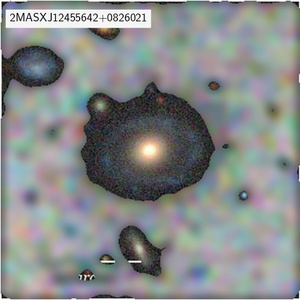
\includegraphics[scale = 0.7]{Images/2MASXJ12455642+0826021.jpg}
    \caption{The starburst event forms a ring of blue gas and star formation around the center, polar with respect to the plane of the galaxy.}
    \label{fig:starburst}
\end{figure}

A final method we discuss in  here (and this list is by no means exhaustive), is accretion from cosmic filaments. As a galaxy passes through filaments in large scale cosmological structures, it may develop polar structures as the intergalactic gas can frictionally force polar structures out of the host galaxy, as seen in figure \ref{fig:cosmic}.

\begin{figure}
    \centering
    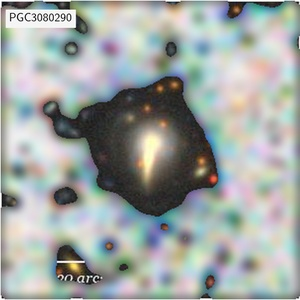
\includegraphics[scale = 0.7]{Images/PGC3080290.jpg}
    \caption{The bulge/core of the galaxy is pressure stripped as it moves through intergalactic gas in a cosmic filament.}
    \label{fig:cosmic}
\end{figure}

Out of the 143 candidates, we can identify 70 'strong' candidates, which we consider to be those candidates that exhibit polar structures with a high confidence interval. 
 

\section{Conclusions}
\label{sec:conclusions}

In this letter, we present the findings from a systematic review over the course of 10 weeks to categorize 143 galaxies with polar structures, 70 of which are highly probable candidates. 
This entails a PRG occurrence rate of about 1.43\%. 
This is highly consistent with the findings of \citet{2024AstL...}, which means the occurrence rate of galaxies with polar structures are much higher than previously thought (\citealt{1990AJ....100.1489W}, \citealt{2011MNRAS.418..244M}). These candidates will be used to train a neural network and conduct a rigorous analysis of polar structure galaxies, based on the largest sample to date. We stress, however, that these galaxies are only candidates for polar structures and are yet to be kinematically confirmed. In a future study, we will release a full catalogue of our polar structure candidates, alongside photometric decompositions of some candidate galaxies identified here. 

\begin{acknowledgements}
Funding for the Sloan Digital Sky Survey IV has been provided by the Alfred P. Sloan Foundation, the U.S. Department of Energy Office of Science, and the Participating Institutions. SDSS-IV acknowledges
support and resources from the Center for High-Performance Computing at the University of Utah. The SDSS website is www.sdss.org.

SDSS-IV is managed by the Astrophysical Research Consortium for the
Participating Institutions of the SDSS Collaboration including the
Brazilian Participation Group, the Carnegie Institution for Science,
Carnegie Mellon University, the Chilean Participation Group, the French Participation Group, Harvard-Smithsonian Center for Astrophysics,
Instituto de Astrof\'isica de Canarias, The Johns Hopkins University, Kavli Institute for the Physics and Mathematics of the Universe (IPMU) /
University of Tokyo, the Korean Participation Group, Lawrence Berkeley National Laboratory,
Leibniz Institut f\"ur Astrophysik Potsdam (AIP),
Max-Planck-Institut f\"ur Astronomie (MPIA Heidelberg),
Max-Planck-Institut f\"ur Astrophysik (MPA Garching),
Max-Planck-Institut f\"ur Extraterrestrische Physik (MPE),
National Astronomical Observatories of China, New Mexico State University,
New York University, University of Notre Dame,
Observat\'ario Nacional / MCTI, The Ohio State University,
Pennsylvania State University, Shanghai Astronomical Observatory,
United Kingdom Participation Group,
Universidad Nacional Aut\'onoma de M\'exico, University of Arizona,
University of Colorado Boulder, University of Oxford, University of Portsmouth,
University of Utah, University of Virginia, University of Washington, University of Wisconsin,
Vanderbilt University, and Yale University.

The Legacy Surveys consist of three individual and complementary projects: the Dark Energy Camera Legacy Survey (DECaLS; NOAO Proposal ID \# 2014B-0404; PIs: David Schlegel and Arjun Dey), the Beijing-Arizona Sky Survey (BASS; NOAO Proposal ID \# 2015A-0801; PIs: Zhou Xu and Xiaohui Fan), and the Mayall z-band Legacy Survey (MzLS; NOAO Proposal ID \# 2016A-0453; PI: Arjun Dey). DECaLS, BASS and MzLS together include data obtained, respectively, at the Blanco telescope, Cerro Tololo Inter-American Observatory, National Optical Astronomy Observatory (NOAO); the Bok telescope, Steward Observatory, University of Arizona; and the Mayall telescope, Kitt Peak National Observatory, NOAO. The Legacy Surveys project is honored to be permitted to conduct astronomical research on Iolkam Du'ag (Kitt Peak), a mountain with particular significance to the Tohono O'odham Nation.

NOAO is operated by the Association of Universities for Research in Astronomy (AURA) under a cooperative agreement with the National Science Foundation.

This project used data obtained with the Dark Energy Camera (DECam), which was constructed by the Dark Energy Survey (DES) collaboration. Funding for the DES Projects has been provided by the U.S. Department of Energy, the U.S. National Science Foundation, the Ministry of Science and Education of Spain, the Science and Technology Facilities Council of the United Kingdom, the Higher Education Funding Council for England, the National Center for Supercomputing Applications at the University of Illinois at Urbana-Champaign, the Kavli Institute of Cosmological Physics at the University of Chicago, Center for Cosmology and Astro-Particle Physics at the Ohio State University, the Mitchell Institute for Fundamental Physics and Astronomy at Texas A\&M University, Financiadora de Estudos e Projetos, Fundacao Carlos Chagas Filho de Amparo, Financiadora de Estudos e Projetos, Fundacao Carlos Chagas Filho de Amparo a Pesquisa do Estado do Rio de Janeiro, Conselho Nacional de Desenvolvimento Cientifico e Tecnologico and the Ministerio da Ciencia, Tecnologia e Inovacao, the Deutsche Forschungsgemeinschaft and the Collaborating Institutions in the Dark Energy Survey. The Collaborating Institutions are Argonne National Laboratory, the University of California at Santa Cruz, the University of Cambridge, Centro de Investigaciones Energeticas, Medioambientales y Tecnologicas-Madrid, the University of Chicago, University College London, the DES-Brazil Consortium, the University of Edinburgh, the Eidgenossische Technische Hochschule (ETH) Zurich, Fermi National Accelerator Laboratory, the University of Illinois at Urbana-Champaign, the Institut de Ciencies de l'Espai (IEEC/CSIC), the Institut de Fisica d'Altes Energies, Lawrence Berkeley National Laboratory, the Ludwig-Maximilians Universitat Munchen and the associated Excellence Cluster Universe, the University of Michigan, the National Optical Astronomy Observatory, the University of Nottingham, the Ohio State University, the University of Pennsylvania, the University of Portsmouth, SLAC National Accelerator Laboratory, Stanford University, the University of Sussex, and Texas A\&M University.

BASS is a key project of the Telescope Access Program (TAP), which has been funded by the National Astronomical Observatories of China, the Chinese Academy of Sciences (the Strategic Priority Research Program "The Emergence of Cosmological Structures" Grant \# XDB09000000), and the Special Fund for Astronomy from the Ministry of Finance. The BASS is also supported by the External Cooperation Program of Chinese Academy of Sciences (Grant \# 114A11KYSB20160057), and Chinese National Natural Science Foundation (Grant \# 11433005).

The Legacy Survey team makes use of data products from the Near-Earth Object Wide-field Infrared Survey Explorer (NEOWISE), which is a project of the Jet Propulsion Laboratory/California Institute of Technology. NEOWISE is funded by the National Aeronautics and Space Administration.

The Legacy Surveys imaging of the DESI footprint is supported by the Director, Office of Science, Office of High Energy Physics of the U.S. Department of Energy under Contract No. DE-AC02-05CH1123, by the National Energy Research Scientific Computing Center, a DOE Office of Science User Facility under the same contract; and by the U.S. National Science Foundation, Division of Astronomical Sciences under Contract No. AST-0950945 to NOAO.

The Hyper Suprime-Cam (HSC) collaboration includes the astronomical communities of Japan and Taiwan, and Princeton University. The HSC instrumentation and software were developed by the National Astronomical Observatory of Japan (NAOJ), the Kavli Institute for the Physics and Mathematics of the Universe (Kavli IPMU), the University of Tokyo, the High Energy Accelerator Research Organization (KEK), the Academia Sinica Institute for Astronomy and Astrophysics in Taiwan (ASIAA), and Princeton University. Funding was contributed by the FIRST program from the Japanese Cabinet Office, the Ministry of Education, Culture, Sports, Science and Technology (MEXT), the Japan Society for the Promotion of Science (JSPS), Japan Science and Technology Agency (JST), the Toray Science Foundation, NAOJ, Kavli IPMU, KEK, ASIAA, and Princeton University.

This paper makes use of software developed for Vera C. Rubin Observatory. We thank the Rubin Observatory for making their code available as free software at http://pipelines.lsst.io/.

This paper is based on data collected at the Subaru Telescope and retrieved from the HSC data archive system, which is operated by the Subaru Telescope and Astronomy Data Center (ADC) at NAOJ. Data analysis was in part carried out with the cooperation of Center for Computational Astrophysics (CfCA), NAOJ. We are honored and grateful for the opportunity of observing the Universe from Maunakea, which has the cultural, historical, and natural significance in Hawaii.

\end{acknowledgements}

\bibliographystyle{aa} % style aa.bst
\bibliography{references}

%%%%%%%%%%%%%%%%%%%%%%%%%%%%%%%%%%%%%%%%%%%%%%%%%%

%%%%%%%%%%%%%%%%%%%%%%%%%%%%%%%%%%%%%%%%%%%%%%%%%%




%%%%%%%%%%%%%%% APPENDICES %%%%%%%%%%%%%%%%%%%%%

\end{document}
